\documentclass[a4paper,12pt]{article}

\usepackage[T2A]{fontenc}
\usepackage[utf8]{inputenc}
\usepackage[english,russian]{babel}
\usepackage{amsmath}
\usepackage{geometry}
\usepackage{graphicx}
\usepackage[section,above,below]{placeins}
\usepackage{afterpage,placeins}
\usepackage{booktabs}
\usepackage{listings}
\usepackage{color}

\usepackage{algorithm}
\usepackage[noend]{algpseudocode}

\DeclareGraphicsExtensions{.png,.jpg}

\geometry{left=2cm}
\geometry{right=1.5cm}
\geometry{top=1cm}
\geometry{bottom=1.5cm}

\headheight = 1cm
\footskip = 0pt
%\usepackage[left=20mm, top=10mm, right=10mm, bottom=5mm, nohead, nofoot]{geometry}

\parskip = 4.25mm % расстояние между строками
\parindent=6.375mm % расстояние между абзацами
\floatname{algorithm}{Алгоритм} % переопределение имени в псевдокоде

%\renewcommand\[{\begin{equation}}
%\renewcommand\]{\end{equation}}

\begin{document}

    \begin{titlepage}

        \begin{center}
            \large
            Государственное образовательное учреждение высшего профессионального образования\\
            “Московский государственный технический университет имени Н.Э.Баумана”
            \vspace{3cm}
            
            \textsc{Дисциплина: Анализ алгоритмов}
            \vspace{0.5cm}
                
            \textsc{Лабораторная работа №3}
            \vspace{3cm}
            
            {\LARGE Сортировки}
            \vspace{3cm}
            
            Студент группы ИУ7-54Б,\\   
            Котов Никита
            \vfill
            
            2019 г.
            
            \end{center}
    \end{titlepage}
    
    \begin{center}
    	\tableofcontents
    \end{center}
	
	\setcounter{page}{2}
	\newpage
    \begin{center}
        \section*{Введение}
        \addcontentsline{toc}{section}{Введение}
    \end{center}
        \label{sec:intro}
\qquad Алгоритм сортировки — это алгоритм для упорядочивания элементов в списке. В случае, когда элемент списка имеет несколько полей, поле, служащее критерием порядка, называется ключом сортировки. На практике в качестве ключа часто выступает число, а в остальных полях хранятся какие-либо данные, никак не влияющие на работу алгоритма.   
		
		
		Первые прототипы современных методов сортировки появились уже в XIX веке. К 1890 году для ускорения обработки данных переписи населения в США американец Герман Холлерит создал первый статистический табулятор — электромеханическую машину, предназначенную для автоматической обработки информации, записанной на перфокартах\cite{litlink1}.
		
		
		Сейчас же сортировки используются повсеместно, и именно им посвящена данная лабораторная работа.\\
В рамках выполнения работы необходимо решить следующие задачи:   
		\begin{itemize}
		    \item рассмотреть и изучить сортировки пузырьком, вставками и выбором;
			\item реализовать каждую из этих сортировок;
			\item рассчитать их трудоемкость; 				
			\item сравнить их временные характеристики экспериментально; 
			\item на основании проделанной работы сделать выводы.
		\end{itemize}
    \newpage

    \begin{center}
        \section{Аналитическая часть}
\subsection{Модель вычислений}
\end{center}


Для последующего вычисления трудоемкости необходимо ввести модель вычислений:
\begin{enumerate}
\item +, -, /, \%, ==, !=, <, >, <=, >=, [], ++, \-- -- имеют трудоемкость 1
\item трудоемкость оператора выбора
			\begin{algorithmic}
			\If{\text{условие}}
				\State A
			\Else
				\State B
			\EndIf
			\end{algorithmic}
 рассчитывается, как 
			\[ f_{if} = f_{\text{условия}} + 
			\begin{cases}
				f_A, & \text{если условие выполняется,}\\
				f_B, & \text{иначе.}
			\end{cases} \]
\item трудоемкость цикла рассчитывается, как $f_{for} = f_{\text{инициализации}} + f_{\text{сравнения}} + N(f_{\text{тела}} + f_{\text{инициализации}} + f_{\text{сравнения}})$
\item трудоемкость вызова метода равна 0
\item трудоемкость вызова функции равна 1
\end{enumerate}

    \newpage
	\begin{center}
	        \subsection{Описание алгоритмов}
    \end{center}
\subsubsection{Сортировка пузырьком}

Алгоритм состоит из повторяющихся проходов по сортируемому массиву. За каждый проход элементы последовательно сравниваются попарно и, если порядок в паре неверный,в ыполняется обмен элементов. Проходы по массиву повторяются N-1 раз или до тех пор, пока на очередном проходе не окажется, что обмены больше не нужны, что означает - массив отсортирован. При каждом проходе алгоритма по внутреннему циклу очередной наибольший элемент массива ставится на свое место в конце массива рядом с предыдущим "наибольшим элементом", а наименьший элемент массива перемещается на одну позицию к началу массива.

\subsection{Сортировка вставками}

Сортировка вставками - алгоритм сортировки, котором элементы входной последовательности просматриваются по одному, и каждый новый поступивший элемент размещается в подходящее место среди ранее упорядоченных элементов\cite{litlink1}.\\
На вход алгоритма подаётся последовательность $n$ чисел:
$a_{1},a_{2},...,a_{n}$. Сортируемые числа также называют ключами.
Входная последовательность на практике представляется в виде массива с $n$ элементами. На выходе алгоритм должен вернуть перестановку
исходной последовательности $a_{1}^{'},a_{2}^{'},...,a_{n}^{'}$,
чтобы выполнялось следующее соотношение $a_{1}^{'}\leq a_{2}^{'}\leq ...\leq a_{n}^{'}$\cite{litlink2}.

В начальный момент отсортированная последовательность пуста. На каждом шаге алгоритма выбирается один из элементов входных данных и помещается на нужную позицию в уже отсортированной последовательности до тех пор, пока набор входных данных не будет исчерпан. В любой момент времени в отсортированной последовательности элементы удовлетворяют требованиям к выходным данным алгоритма\cite{litlink2}. 

\subsection{Сортировка выбором}

Шаги алгоритма:
\begin{enumerate}
    \item находим номер минимального значения в текущем списке
    \item производим обмен этого значения со значением первой неотсортированной позиции (обмен не нужен, если минимальный элемент уже находится на данной позиции)
    \item теперь сортируем хвост списка, исключив из рассмотрения уже отсортированные элементы
\end{enumerate}
Для реализации устойчивости алгоритма необходимо в пункте 2 минимальный элемент непосредственно вставлять в первую неотсортированную позицию, не меняя порядок остальных элементов. 

    \newpage

    \begin{center}
        \section{Конструкторская часть}
        \subsection{Разработка алгоритмов}
        \subsubsection{Сортировка пузырьком}
    \end{center}
    На рис.~\ref{ris:rec_sheme} представлена схема сортировки пузырьком
		 		\begin{figure}[h]
		 			\centering
		 			{
		 				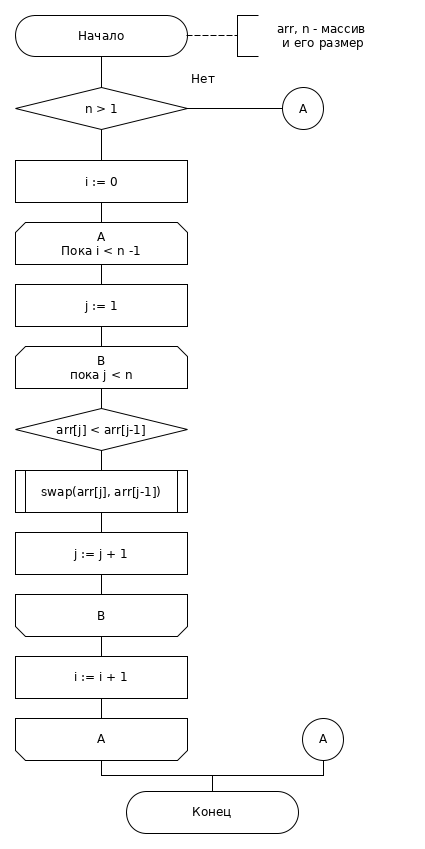
\includegraphics[scale=0.51]{buble.png}
		 				\caption{Сортировка пузырьком}
			 			\label{ris:rec_sheme}
		 			}
		 		\end{figure}
	
	Лучшим случаем является ситуация, когда массив уже отсортирован, так как количество произведенных обменов будет равно 0.\\
	Худшим же случаем является обратно отсортированный массив, так как обмен будет выполняться на каждом шаге.\\
	Оценим трудоемкость:
	\begin{itemize}
		\item Худший случай(неотсортированный массив): $3 + (n - 1)(5 + 13(n-1)) = 13n^{2}-21n+11 \sim O(n^{2})$
		\item Лудший случай(отсортированный массив): $3 + (n - 1)(5 + 6(n - 1) = 6n^{2}-7n+1 \sim O(n^{2})$
	\end{itemize}
    \newpage
    \afterpage{\FloatBarrier}
    \subsubsection{Сортировка вставками}
        На рис.~\ref{ris:matr_lev_sh1} представлена схема сортировки вставками
		 		\begin{figure}[H]
		 			\centering
		 			{
		 				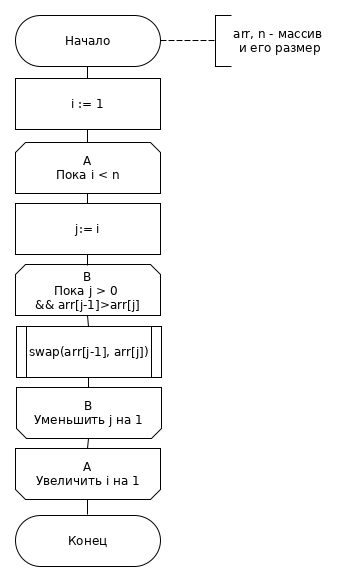
\includegraphics[scale=0.51]{insert.png}
		 				\caption{Сортировка вставками}
		 				\label{ris:matr_lev_sh1}
		 			}
		 		\end{figure}		 	
	Лучшим случаем является предварительно отсортированный массив, так как тогда требуется только один проход по массиву и не производятся перестановки.\\
	Худшим случаем является обратно отсортированный массив, т.к. при этом производится максимально возможное количество обменов.	
	Трудоемкость алгоритма в лучшем случа $O(n)$, в худшем - $O(n^{2})$\cite{litlink1}.
    \newpage
    \afterpage{\FloatBarrier}
    \subsubsection{Сортировка выбором}
            На рис.~\ref{ris:matr_dl_sh1} представлена схема сортировки выбором
            
\begin{figure}[H]
		 			\centering
		 			{
		 				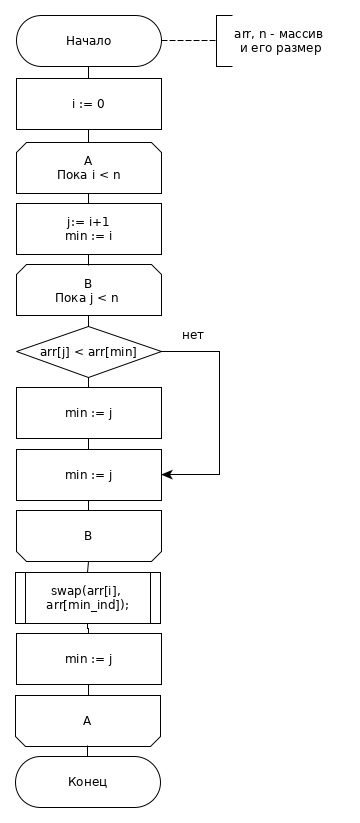
\includegraphics[scale=0.51]{select.png}
		 				\caption{Сортировка выбором}
		 				\label{ris:matr_dl_sh1}
		 			}
		 		\end{figure}
	Лучшим случаем является отсортированный массив, так как при этом выполняется 1 операцию присваивания меньше на каждой итерации.\\
	Худшим же обратно отсортированный массив, на каждой итерации выполняется на 1 операцию больше по сравнению с лучшим случаем.
	Трудоемкость алгоритма в обоих случаях составляет $O(n^{2})$\cite{litlink1}
    \newpage
    \afterpage{\FloatBarrier}
    
    
    \begin{center}
    	\subsection{Выводы по конструкторскому разделу}    
    \end{center}
   
    	\qquad Были разработаны схемы всех трех алгоритмов сортировки. Для каждого из них были выделены и оценены лучшие и худшие случаи
    	
    \newpage
    
    \begin{center}
     	\section{Технологическая часть}    	
        \subsection{Средства реализации}    
    \end{center}
    
		В качестве языка программирования был выбран C++, так как он предоставляет широкие возможности для эффективной реализации алгоритмов.
	\begin{center}
	\end{center}
	\begin{center}
		\subsection{Структура программы}	
		\end{center}
	
    	\noindent sort.cpp - содержит реализации алгоритмов сортировок\\
    	test.cpp - содержит тесты для реализованных алгоритмов\\
	    main.cpp - содержит интерфейс для взаимодействия с программой\\
		\newpage
    \begin{center}
        \subsection{Листинг кода}    
    \end{center}
\lstset{
        		language=C++,
        		basicstyle=\ttfamily,
        		keywordstyle=\color{blue}\ttfamily,
        		stringstyle=\color{red}\ttfamily,
        		commentstyle=\color{green}\ttfamily,
        		morecomment=[l][\color{magenta}]{\#},
        		columns=fullflexible,
        	    tabsize=1, 
        		breakatwhitespace=true
}
        	
\begin{lstlisting}[frame=single,caption=Сортировка пузырьком, breaklines]
void bubble_sort(std::vector<double> &arr) {
    if (arr.empty()) {
        return;
    }

    for (int i = 0; i < arr.size() - 1; i++) {
        for (int j = 1; j < arr.size(); j++) {
            if (arr[j] < arr[j - 1]) {
                std::swap(arr[j - 1], arr[j]);
            }
        }
    }
}
        		\end{lstlisting}        		
    
\begin{lstlisting}[frame=single,caption=Сортировка вставками, breaklines]
void insertion_sort(std::vector<double> &arr) {
    if (arr.empty()) {
        return;
    }

    for (size_t i = 1; i < arr.size(); i++) {
        auto cur_item = arr[i];
        int j = static_cast<int>(i - 1);
        for (; j >= 0 && arr[j] > cur_item; j--) {
            arr[j + 1] = arr[j];
        }
        arr[j + 1] = cur_item;
    }
}
\end{lstlisting}

\begin{lstlisting}[frame=single,caption=Сортировка выбором, breaklines]
void choice_sort(std::vector<double> &arr) {
    if (arr.empty()) {
        return;
    }

    for (size_t i = 0; i < arr.size() - 1; i++) {
        auto min_ind = i;
        for (size_t j = i + 1; j < arr.size(); j++) {
            if (arr[j] < arr[min_ind]) {
                min_ind = j;
            }
        }
        std::swap(arr[min_ind], arr[i]);
    }
}
\end{lstlisting}
    \newpage

    \begin{center}
		\subsection{Тестирование фунций}
	\end{center}
		\quadВ таблице ~\ref{tabular:test_rec}, таблице~\ref{tabular:test_mtrx_l}, таблице~\ref{tabular:test_mtrx_dl} приведены результаты тестирования для сортировок пузырьком, вставками и выбором соответственно.
        			\begin{table}[H]        		
       				\caption{\label{tabular:test_rec} Сортировка пузырьком}
       				\begin{center}       			
        			\begin{tabular}{|c|c|c|}        				
        				\hline
						Входной массив & Результат & Ожидаемый результат \\ 
						\hline
        				$[1,2,3,4]$ & $[1,2,3,4]$  & $[1,2,3,4]$\\
        				$[3,2,1]$  & $[1,2,3]$ & $[1,2,3]$\\
        				$[5,6,2,4,-2]$  & $[-2,2,4,5,6]$  & $[-2,2,4,5,6]$\\
        				$[4]$  & $[4]$  & $[4]$\\
        				$[]$  & $[]$  & $[]$\\
        				\hline
        			\end{tabular}
       				\end{center}
        			\end{table}        			
        			\vspace{1cm}
        		
        			\begin{table}[H]        		
       				\caption{\label{tabular:test_mtrx_l} Сортировка вставками}
       				\begin{center}
        			\begin{tabular}{|c|c|c|}        				
        				\hline
						Входной массив & Результат & Ожидаемый результат \\ 
						\hline
        				$[1,2,3,4]$ & $[1,2,3,4]$  & $[1,2,3,4]$\\
        				$[3,2,1]$  & $[1,2,3]$ & $[1,2,3]$\\
        				$[5,6,2,4,-2]$  & $[-2,2,4,5,6]$  & $[-2,2,4,5,6]$\\
        				$[4]$  & $[4]$  & $[4]$\\
        				$[]$  & $[]$  & $[]$\\
        				\hline
        			\end{tabular}
        			\end{center}
        			\end{table}
        			\vspace{1cm}
        		
					\begin{table}[H]        		
       				\caption{\label{tabular:test_mtrx_dl} Сортировка выбором}
       				\begin{center}       			
        			\begin{tabular}{|c|c|c|}        				
        				\hline
						Входной массив & Результат & Ожидаемый результат \\ 
						\hline
        				$[1,2,3,4]$ & $[1,2,3,4]$  & $[1,2,3,4]$\\
        				$[3,2,1]$  & $[1,2,3]$ & $[1,2,3]$\\
        				$[5,6,2,4,-2]$  & $[-2,2,4,5,6]$  & $[-2,2,4,5,6]$\\
        				$[4]$  & $[4]$  & $[4]$\\
        				$[]$  & $[]$  & $[]$\\
        				\hline
        			\end{tabular}
     	 				\end{center}
	        		\end{table}
	\newpage

    \begin{center}
        \section{Экспериментальная часть}        
	    \subsection{Тестирование времени работы функций}	
	\end{center}
	    \quadДля измерения времени использовалась функция clock(). Чтобы исключить случайные отклонения в измеренном времени, измерялось время работы 10 запусков функции и делилось на 10.
	    
	    В таблице~\ref{tabular:test_time1} представлены результаты замеров времени работы сортировок на отсортированных массивах, в таблице~\ref{tabular:test_time2} на обратно отсортированных и в таблице~\ref{tabular:test_time3}. На рис.~\ref{ris:cmp_mtrx} и рис.~\ref{ris:cmp_r_and_m} изображены графики, позволяющие наглядно сравнить эффективность реализованных алгоритмов сортировок.
	    
	\begin{table}[H]
	\caption{\label{tabular:test_time1} Время работы на отсортированных массивах}
	\begin{center}	    
	\begin{tabular}{|c|c|c|c|}        				
        				\hline
        				Размер массива & Пузырек & Вставки & Выбор       \\ 
        				\hline
        				100    &0.0000760 &0.0000002 &0.0000042\\ 
        				500    &0.0001662 &0.0000016 &0.0000888\\
        				1000   &0.0006588 &0.0000017 &0.0003322\\ 
        				5000   &0.0186644 &0.0000084 &0.0082122\\
        				20000  &0.2670918 &0.0000312 &0.1332514\\
        				50000  &1.8965828 &0.0000656 &0.8430474\\
        				\hline
	\end{tabular}
	\end{center}
	\end{table}	

	\begin{table}[H]
	\caption{\label{tabular:test_time2} Время работы на обратно отсортированных массивах}
	\begin{center}	    
	\begin{tabular}{|c|c|c|c|}        				
        				\hline
        				Размер массива & Пузырек & Вставки & Выбор       \\ 
        				\hline
        				100    &0.0000106 &0.0000018 &0.0000054\\ 
        				500    &0.0001930 &0.0000198 &0.0000878\\
        				1000   &0.0007774 &0.0000754 &0.0003400\\ 
        				5000   &0.0190598 &0.0019278 &0.0085574\\
        				20000  &0.3052872 &0.0299092 &0.1368812\\
        				50000  &1.8856402 &0.1933902 &0.8473344\\
        				\hline
	\end{tabular}
	\end{center}
	\end{table}
	
	\begin{table}[H]
	\caption{\label{tabular:test_time3} Время работы на произвольных массивах}
	\begin{center}	    
	\begin{tabular}{|c|c|c|c|}        				
        				\hline
        				Размер массива & Пузырек & Вставки & Выбор       \\ 
        				\hline
        				100    &0.0000106 &0.0000014 &0.0000058\\ 
        				500    &0.0001946 &0.0000114 &0.0000964\\
        				1000   &0.0007532 &0.0000446 &0.0003844\\ 
        				5000   &0.0207424 &0.0009334 &0.0082266\\
        				20000  &0.3687078 &0.0156806 &0.1322612\\
        				50000  &2.3855662 &0.0933284 &0.8455662\\
        				\hline
	\end{tabular}
	\end{center}
	\end{table}
		
	\begin{center}
	\begin{figure}[H]	
	{
		\centering
      	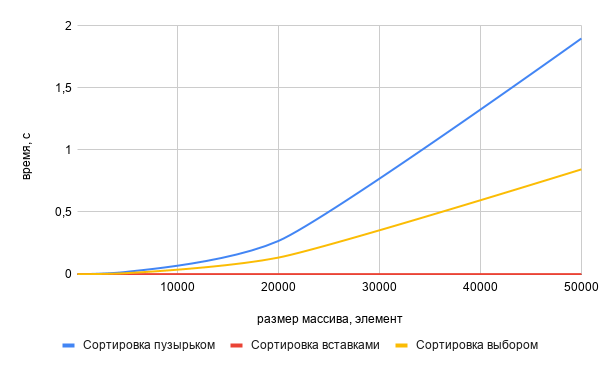
\includegraphics[scale=0.7]{chart.png}
        \caption{Сравнение сортировок на отсортированных массивах}
        \label{ris:cmp_mtrx}
    }
    \end{figure}
        		
	\begin{figure}[H]	
    {
    	\centering
    	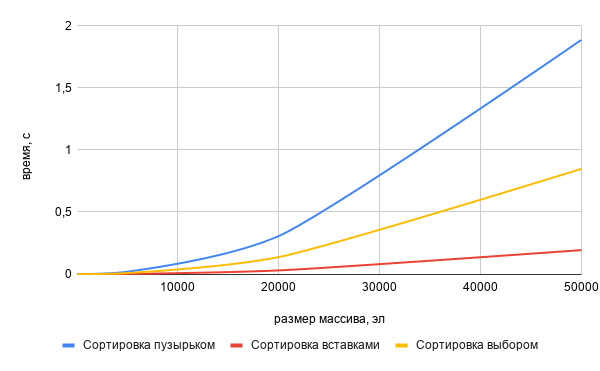
\includegraphics[scale=0.7]{chart1.png}
    	\caption{\label{ris:cmp_r_and_m}Сравнение сортировок на обратно отсортированных массивах}        					
    }
    \end{figure}
    
    \begin{figure}[H]	
	{
		\centering
		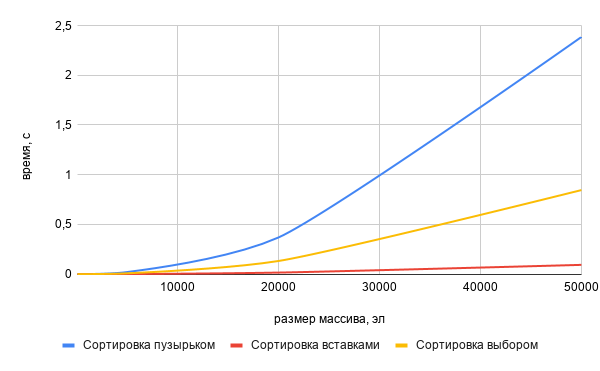
\includegraphics[scale=0.7]{chart2.png}
		\caption{\label{ris:cmp_r_and_m}Сравнение сортировок на произвольных массивах}        					
	}
	\end{figure}
	\end{center}

	На графиках видно, что наиболее эффективным алгоритмом является сортировка вставками, на произвольных массивах она на $\sim95\%$ быстрее остальных. Сортировка выбором на $\sim80\%$ быстрее пузырьково сортировки.

    \newpage

    \begin{center}
        \section*{Заключение}
        \addcontentsline{toc}{section}{Заключение}
    \end{center}
            \label{sec:ending}
        	\qquad В рамках лабораторной работы были реализованы и изучены сортировки пузырьком, вставками и выбором. Была оценена их трудоемкость, произведены замеры времени работы реализованных алгоритмов и сравнена их эффективность по времени. Наиболее эффективной оказалась сортировка вставками, выигрывая по времени на $\sim95\%$ у пузырьковой и на $\sim80\%$ у сортировки вставками, особенно эффективна же она на отсортированных массивах, т.к. работает за линейное время.

    \newpage

    \begin{center}        
        \begin{thebibliography}{}
        	\bibitem{litlink1}  Кнут Д. Э. Искусство программирования. Том 3. Сортировка и поиск = The Art of Computer Programming. Volume 3. Sorting and Searching / под ред. В. Т. Тертышного (гл. 5) и И. В. Красикова (гл. 6). — 2-е изд. — Москва: Вильямс, 2007. — Т. 3. — 832 с. — ISBN 5-8459-0082-1.
        	\bibitem{litlink2} Кормен, Т., Лейзерсон, Ч., Ривест, Р., Штайн, К. 2.1. Сортировка вставкой // Алгоритмы: построение и анализ = Introduction to Algorithms / Под ред. И. В. Красикова. — 3-е изд. — М.: Вильямс, 2013. — С. 38—45. — ISBN 5-8459-1794-8.
        \end{thebibliography}
    \end{center}

\end{document}
